\section{Crowdsourcing Task Interfaces}\label{sec:crowdsourcing_task_interfaces}
In this section some example interfaces are presented which were shown to crowd workers for each verification task. 

After selecting the concepts for ontology validation, the plugin automatically creates the relevant crowdsourcing jobs. Only Figure~Eight is currently supported as target crowdsourcing platform. Depending on the method of context enrichment~(see \hyperref[chap:context_enrichment_methods]{Chapter~\ref*{chap:context_enrichment_methods}}) different crowdsourcing interfaces were generated, as illustrated in \hyperref[fig:all_crowdsourcing_interfaces]{Figure~\ref*{fig:all_crowdsourcing_interfaces}}. 

\begin{figure}
    \centering
    \begin{subfigure}[b]{\textwidth}
        
\includegraphics[width=\textwidth]{screenshots/questionaire_subclass_relation_context_enrichment}
        \caption{Neighbouring Nodes}
        \label{fig:crowdsourcing_interface_nn}
    \end{subfigure}
	~\\~\\
    \begin{subfigure}[b]{\textwidth}
        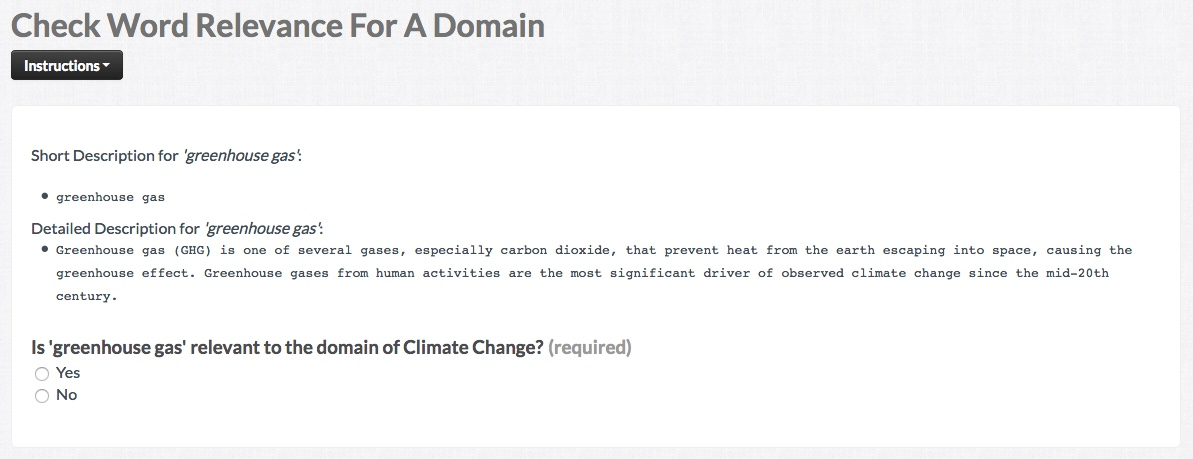
\includegraphics[width=\textwidth]{screenshots/questionaire_embedded_context_enrichment}
        \caption{Embedded Context}
        \label{fig:crowdsourcing_interface_ec}
    \end{subfigure}
	~\\~\\
    \begin{subfigure}[b]{\textwidth}
        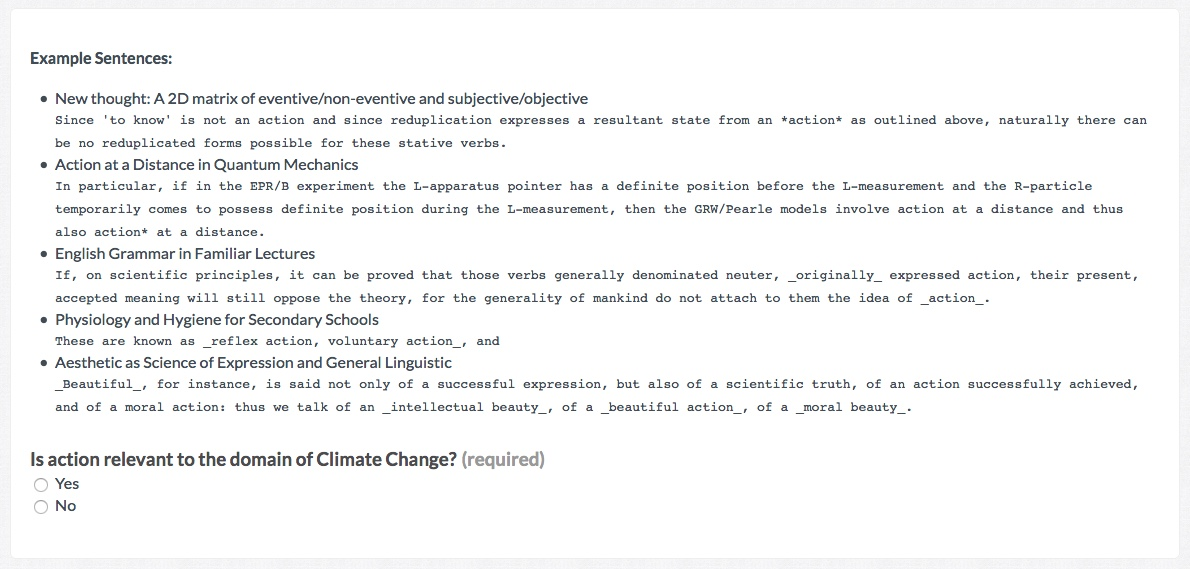
\includegraphics[width=\textwidth]{screenshots/questionaire_wordnik_context_enrichment}
        \caption{External Source}
        \label{fig:crowdsourcing_interface_es}
    \end{subfigure}
    \caption{Crowdsourcing task interfaces for performing ontology validation using different methods of context enrichment}\label{fig:all_crowdsourcing_interfaces}
\end{figure}

Each crowdsourcing interface consists of
\begin{enumerate}
		\item the instruction part
		\item the context part
		\item the question part
\end{enumerate}

The \emph{instructions} are very generic and therefore independent of the chosen context enrichment method. It contains a short description of the task goals and some examples of already answered verification questions. We paid attention to omit the details of ontology validation because first, it would confuse contributors and second, it is not relevant for answering the question. Also, we advised them to browse the Web or contact Wikipedia in case they do not know the answer or are unsure. It encourages contributors to give answers to their best knowledge and increases the quality of the responses at the same time. 

The \emph{context part} is adjusted based on the context enrichment method.
In \hyperref[fig:crowdsourcing_interface_nn]{Figure~\ref*{fig:crowdsourcing_interface_nn}}, the context description is generated by the \emph{Neighbouring Nodes} method, whereas each statement corresponds to a relation. In this example, the concept \emph{fusion} is related to 3 other concepts by subsumption: $ fusion$  \emph{subclassOf} $ \{ heat, action \} $ and $ state $ \emph{subclassOf} $ fusion $. As of now, only subsumption relations are taken into account for the generation of context descriptions. 
\hyperref[fig:crowdsourcing_interface_ec]{Figure~\ref*{fig:crowdsourcing_interface_ec}} displays the generated context description for the concept \emph{greenhouse~gas}. It contains the short description as well as the detailed description, which were previously added by domain experts.
\hyperref[fig:crowdsourcing_interface_es]{Figure~\ref*{fig:crowdsourcing_interface_es}} shows some example sentences for the concept \emph{action} which were obtained from an \emph{External Source}. Thereby each sentence is prepended by a headline written in bold letters. Currently, the plugin only supports WordNik as sentence provider. 

The \emph{question part} contains the actual question which crowd workers had to answer. To prevent spamming, we added a minimum time of $10$ seconds to answer the question. Due to the suggestive nature of the questions, contributors can not skip certain questions in case of uncertainty. This ensures completeness of the result set on the one hand, but also has the potential to produce wrong or incorrect answers. 

